
As a starting example, we consider a compartment pharmacokinetic model for a single patient.
The patient receives multiple doses at regular time intervals and the drug plasma concentration is recorded over time.
Our goal is to infer the physiological parameters of the patient, pertinent to the drug's pharmacokinetics, and the measurement error.

\subsection{Nonlinear pharmacokinetic / pharmacodynamic model} 
For the last example, let us go back to the single patient
two-compartment model and append it with a PD
model. Specifically, we examine the
Friberg-Karlsson semi-mechanistic model for drug-induced
myelosuppression [27, 28, 29, 30, 31, 14] with the goal to model the
relation between neutrophil counts and drug exposure.
It describes a delayed feedback mechanism that keeps the absolute neutrophil count (ANC) at the
baseline ($\text{Circ}_0$) in a circulatory compartment ($y_{\text{circ}}$), as well as the drug
effect that perturbs this meachanism. The delay between
proliferative cells ($y_{\text{prol}}$) and $y_{\text{circ}}$ is modeled by three
transit compartments with mean transit time
\begin{equation}
  \text{MTT} = (3 + 1)/k_{\text{tr}}
\end{equation}
where $k_{\text{tr}}$ is the transit rate constant.
\begin{figure}
  \begin{center}
  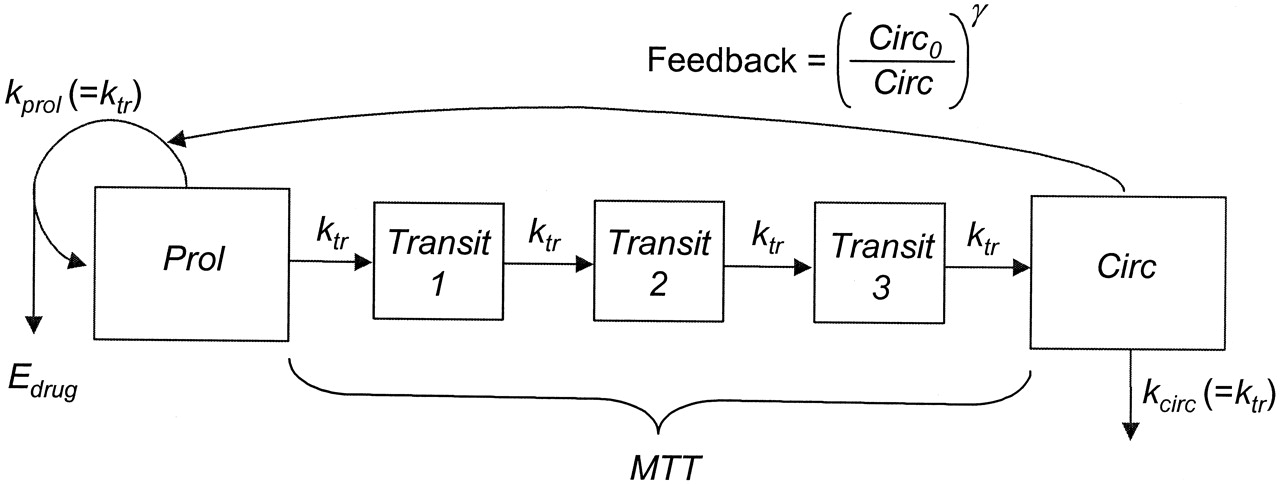
\includegraphics[width=5in]{../figures/neutrophilModel.jpg}
  \caption{Friberg-Karlsson semi-mechanistic Model.}
  \label{fig:fk_model}
  \end{center}
\end{figure}

The PD model can be summarized as
\begin{align*}
  \log(\text{ANC})& \sim N(\log(y_{\text{circ}}), \sigma^2_{\text{ANC}}),  \\
  y_{\text{circ}}& = f_{\text{FK}}(\text{MTT}, \text{Circ}_{0}, \alpha, \gamma, c),
  % (\text{MTT}, \text{Circ}_{0}, \alpha, \gamma, k_{\text{tr}})& = (125, 5.0, 3 \times 10^{-4}, 0.17) \\
  % \sigma^2_{\text{ANC}}& = 0.001
\end{align*}
where \(c\) is the pasma drug concentration calculated from the PK model, and function $f_{\text{FK}}$ represents solving  the following
nonlinear ODE for $y_{\text{circ}}$ 
\begin{subequations}\label{eq:FK}
\begin{align}
  \frac{dy_\mathrm{prol}}{dt} &= k_\mathrm{prol} y_\mathrm{prol} (1 - E_\mathrm{drug})\left(\frac{\text{Circ}_0}{y_\mathrm{circ}}\right)^\gamma - k_\mathrm{tr}y_\mathrm{prol}, \\
  \frac{dy_\mathrm{trans1}}{dt} &= k_\mathrm{tr} y_\mathrm{prol} - k_\mathrm{tr} y_\mathrm{trans1}, \\
  \frac{dy_\mathrm{trans2}}{dt} &= k_\mathrm{tr} y_\mathrm{trans1} - k_\mathrm{tr} y_\mathrm{trans2},  \\
  \frac{dy_\mathrm{trans3}}{dt} &= k_\mathrm{tr} y_\mathrm{trans2} - k_\mathrm{tr} y_\mathrm{trans3},  \\
  \frac{dy_\mathrm{circ}}{dt} &= k_\mathrm{tr} y_\mathrm{trans3} - k_\mathrm{tr} y_\mathrm{circ},
\end{align}
\end{subequations}
We use $E_{\text{drug}} = \alpha c$ to model the linear effect of drug
concentration in central compartment that reduces the proliferation rate or induces cell loss. The entire ODE system is formed by coupling equation \eqref{eq:twocpt}
and \eqref{eq:FK}, with
$c=y_{\text{cent}}/V_{\text{cent}}$ based on PK solution.
The following \texttt{parameters} block summarizes the unknown parameters this model
\begin{lstlisting}[style=stan, numbers=none] 
parameters{
  // PK parameters
  real<lower = 0> CL;
  real<lower = 0> Q;
  real<lower = 0> V1;
  real<lower = 0> V2;
  real<lower = 0> ka;

  // PD parameters
  real<lower = 0> mtt;       // mean transit time
  real<lower = 0> circ0;     // baseline
  real<lower = 0> alpha;     // linear drug effect coefficient
  real<lower = 0> gamma;     // feedback effect exponent
  real<lower = 0> sigma;     // sd for drug concentration likelihood
  real<lower = 0> sigmaNeut; // sd for neutrophil count likelihood
}
\end{lstlisting}

Unlike in
Section \ref{sec:twocpt}, here to solve the nonlinear system we must
utilize one of the numerical solvers in Torsten.

\subsubsection{Numerical solution of ODE}
To solve an ODE numerically in Stan we first need to define
its right-hand-side in the \texttt{functions} block.
\begin{lstlisting}[style=stan, numbers=none] 
functions {
  real[] twoCptNeutModelODE(real t, real[] y, real[] parms, real[] rdummy, int[] idummy){
    real CL = parms[1];
    real Q = parms[2];
    real V1 = parms[3];
    real V2 = parms[4];
    real ka = parms[5];
    real mtt = parms[6];	
    real circ0 = parms[7];
    real gamma = parms[8];
    real alpha = parms[9];
    real k10 = CL / V1;
    real k12 = Q / V1;
    real k21 = Q / V2;
    real ktr = 4 / mtt;
    real dydt[8];
    real conc = y[2]/V1;
    real EDrug = fmin(1.0, alpha * conc);
    real prol = y[4] + circ0;
    real transit1 = y[5] + circ0;
    real transit2 = y[6] + circ0;
    real transit3 = y[7] + circ0;
    real circ = fmax(machine_precision(), y[8] + circ0);

    dydt[1] = -ka * y[1];
    dydt[2] = ka * y[1] - (k10 + k12) * y[2] + k21 * y[3];
    dydt[3] = k12 * y[2] - k21 * y[3];

    // y[4] - y[8] are differences from baseline circ0.
    dydt[4] = ktr * prol * ((1 - EDrug) * ((circ0 / circ)^gamma) - 1);
    dydt[5] = ktr * (prol - transit1);
    dydt[6] = ktr * (transit1 - transit2);
    dydt[7] = ktr * (transit2 - transit3);
    dydt[8] = ktr * (transit3 - circ);

    return dydt;
  }
}
\end{lstlisting}
In this example, we solve the defined ODE in \texttt{transformed parameters}
using the Runge-Kutta solver \texttt{pmx\_solve\_rk45}.
\begin{lstlisting}[style=stan, numbers=none] 
transformed parameters{
  vector[nt] cHat;
  vector[nObsPK] cHatObs; // predictions for observed data
  vector[nt] neutHat;
  vector[nObsPD] neutHatObs; // predictions for observed data
  matrix[8, nt] y;
  real<lower = 0> parms[9];

  parms = {CL, Q, V1, V2, ka, mtt, circ0, gamma, alpha};

  y = pmx_solve_rk45(twoCptNeutModelODE, nCmt, time, amt, rate, ii, evid, cmt, addl, ss, parms, F, tLag, rtol, atol, max_num_step);

  cHat = y[2, ]' / V1;
  neutHat = y[8, ]' + circ0;

  cHatObs = cHat[iObsPK];
  neutHatObs = neutHat[iObsPD];
}
\end{lstlisting}
Like \texttt{pmx\_solve\_twocpt}, we supply events specification to the \texttt{pmx\_solve\_rk45} function call.
In fact here we also provide bioavailabity fraction \texttt{F} and dosing lag
time \texttt{tLag}, despite the fact that they are defined with default values
therefore can be omitted.
\begin{lstlisting}[style=stan, numbers=none] 
transformed data{
  // ....
  int<lower = 1> nCmt = 8;  // dimension of ODE system
  real F[nCmt] = rep_array(1.0, nCmt);
  real tLag[nCmt] = rep_array(0.0, nCmt);
}
\end{lstlisting}
In the rest of the section we omit the code in other blocks that are similar to what we have
introduced and focus on where user should pay attention to when employing numerical ODE solvers.

First, note that \texttt{pmx\_solve\_rk45}
requires a user-defined ODE function as the first argument (similar to
how one solve an ODE using Stan function \texttt{ode\_rk45}),
and the dimension of the ODE system as the second. More importantly,
despite Stan/Torsten provides default values, we highly recommend user
judiciously choose control parameters
\begin{itemize}
\item \texttt{rtol}: relative tolerance to determine solution convergence,
\item \texttt{atol}: absolute tolerance to determine solution convergence,
\item \texttt{max\_num\_step}: maximum allowed steps.
\end{itemize}
In particular, user should make problem-dependent decision on \texttt{rtol} and \texttt{atol},
according to estimated scale of the unknowns, so that the error would
not affect inference on statistical variance of quantities that enter
the Stan model. For example, when an unknown can be neglected below
certain threshold without affecting the rest of the dynamic system,
setting \texttt{atol} greater than that threshold will avoid spurious and
error--prone computation.

\subsubsection{Solve PKPD model as coupled ODE system}
An acute observer may have noticed that the above combined PKPD model
exhibits an one-way coupling. That is, the PK (Eq. \eqref{eq:twocpt})
has no dependence on the PD (Eq. \eqref{eq:FK}): the PK and PD are
coupled through the proliferation cell count
$y_{\text{prol}}$ and $E_{\text{drug}}$. Frequent encounter with this
type of models is the motivation behind Torsten's coupled solvers.
Such a solver first solves PK analytically, then
passes the PK solution to the PD system and seeks its numerical
solution. Since the dimension numerical ODE solution is reduced, in general this coupled strategy is more efficient than
solving a full ODE system as we did in the last section.
To see it in action, let us apply the
coupled solver \texttt{pmx\_solve\_twocpt\_rk45} to the same drug-induced
myelosuppression model. We need only make two changes. First, to
modify the ODE function to reflect that only the PD states are to be solved.
\begin{lstlisting}[style=stan, numbers=none] 
functions{
  real[] twocptneutmodelode(real t, real[] y, real[] y_pk, real[] theta, real[] rdummy, int[] idummy){
    /* PK variables */
    real V1 = theta[3];

    /* PD variable */
    real mtt      = theta[6];
    real circ0    = theta[7];
    real alpha    = theta[8];
    real gamma    = theta[9];
    real ktr      = 4.0 / mtt;
    real prol     = y[1] + circ0;
    real transit1 = y[2] + circ0;
    real transit2 = y[3] + circ0;
    real transit3 = y[4] + circ0;
    real circ     = fmax(machine_precision(), y[5] + circ0);
    real conc     = y_pk[2] / V1;
    real EDrug    = alpha * conc;

    real dydt[5];

    dydt[1] = ktr * prol * ((1 - EDrug) * ((circ0 / circ)^gamma) - 1);
    dydt[2] = ktr * (prol - transit1);
    dydt[3] = ktr * (transit1 - transit2);
    dydt[4] = ktr * (transit2 - transit3);
    dydt[5] = ktr * (transit3 - circ);

    return dydt;
  }
}
\end{lstlisting}
Note that here we pass in PK and PD states as separate arguments $y$
and $y_{\text{PK}}$, and the function describes the ODE for $y$, while
$y_{\text{PK}}$ will be solved in the backstage.

Then we can simply replace \texttt{pmx\_solve\_rk45} with
\texttt{pmx\_solve\_twocpt\_rk45}.
\begin{lstlisting}[style=stan, numbers=none] 
transformed parameters{
// ...
  x = pmx_solve_twocpt_rk45(twocptneutmodelode, nOde, time, amt, rate, ii, evid, cmt, addl, ss, parms, biovar, tlag, rtol, atol, max_num_step);
// ...
}
\end{lstlisting}
